\subsection{\label{subsec:FZV6}Dispersion von Glas}
Glas absorbiert insbesondere im UV-Bereich $\lambda < \SI[]{250}{\nano\metre}$ und wieder im langwelligen Bereich. Im sichtbaren Spektralbereich hingegen absorbiert Glas kaum. Ein Transmissionsspektrum von Quartz-Glas und Fensterglas ist in Abb.~\ref{fig:glasabs} zu sehen.

\begin{figure}
    \centering
    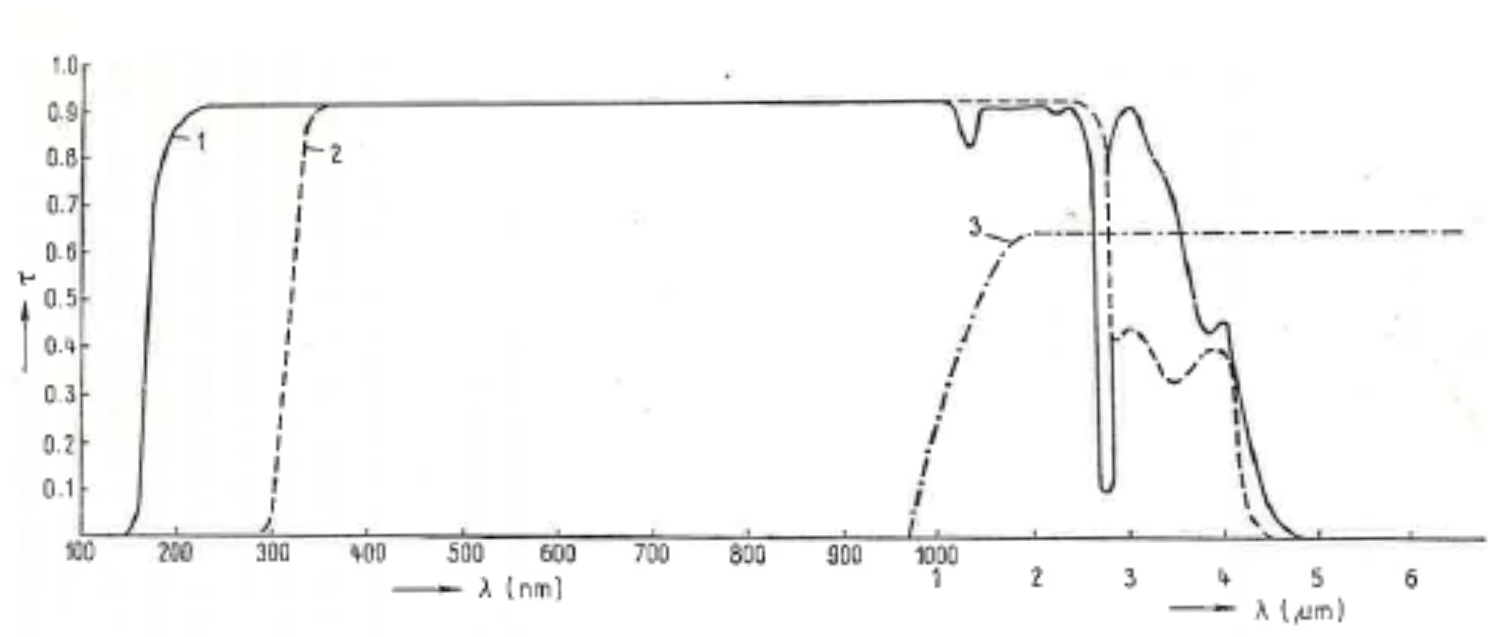
\includegraphics[width=0.5\textwidth]{glas_spektrum1.png}
    \caption{Transmissionsspektrum von Quartz-Glas (1), Fensterglas (2) und Chalcogenid-Glas (3) aus~\cite{glass}. Die Absorptionskanten sind klar erkennbar.}
    \label{fig:glasabs}
\end{figure}

Der Dispersionsverlauf von Glas ist in Abb.~\ref{fig:glasdisp} zu sehen. Wie man sieht ist der Brechungsindex im sichtbaren Spektralbereich nahezu konstant, abgesehen davon jedoch stark von der Wellenlänge abhängig.

\begin{figure}
    \centering
    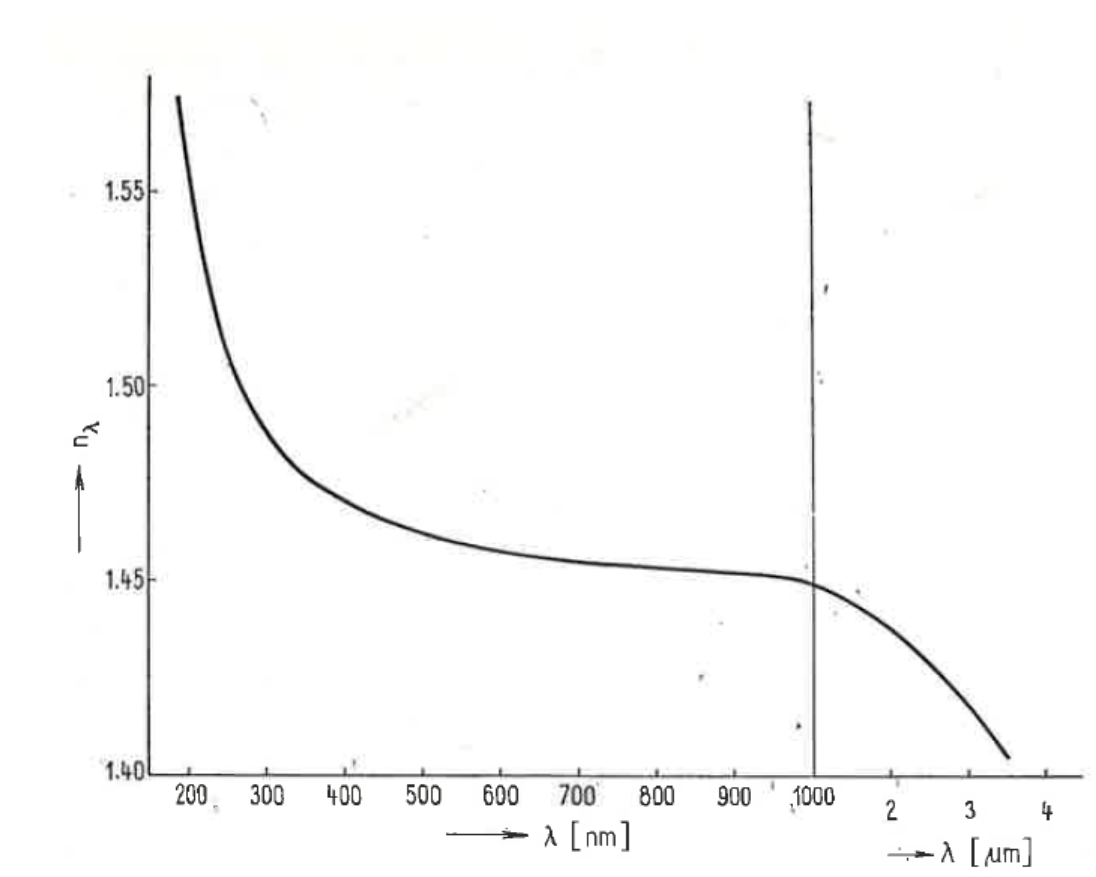
\includegraphics[width=0.5\textwidth]{glas_dispersion1.png}
    \caption{Dispersionsrelation von Quartz-Glas aus~\cite{glass}.}
    \label{fig:glasdisp}
\end{figure}

Silizium absorbiert insbesondere stark in Bereichen $\lambda < \SI[]{1000}{\nano\metre}$, also sowohl im sichtbaren als auch besonders im UV-Bereich. Das Absorptionsspektrum von Silizium ist in Abb.~\ref{fig:siliziumabs} zu sehen.  

\begin{figure}
    \centering
    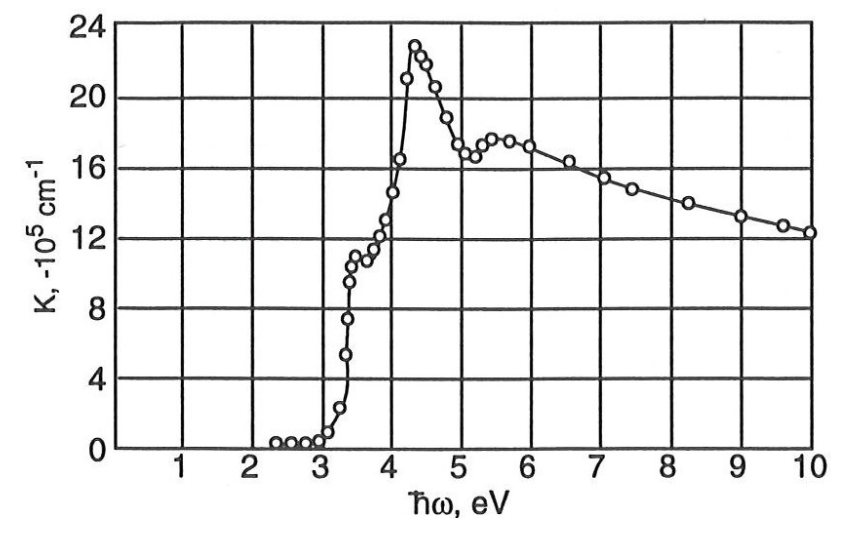
\includegraphics[width=0.4\textwidth]{sil_spektrum1.png}
    \caption{Transmissionsspektrum von Silizium aus~\cite{silicon}. Statt Wellenlängen und Absorption in \% sin dhier Absorptionskoeffizient gegen Energie mit Frequenz $\omega$ aufgetragen.}
    \label{fig:siliziumabs}
\end{figure}

Die Dispersionsrelation und damit die Bandstruktur von Silizium ist in Abb.~\ref{fig:sildisp} zu sehen. 

\begin{figure}
    \centering
    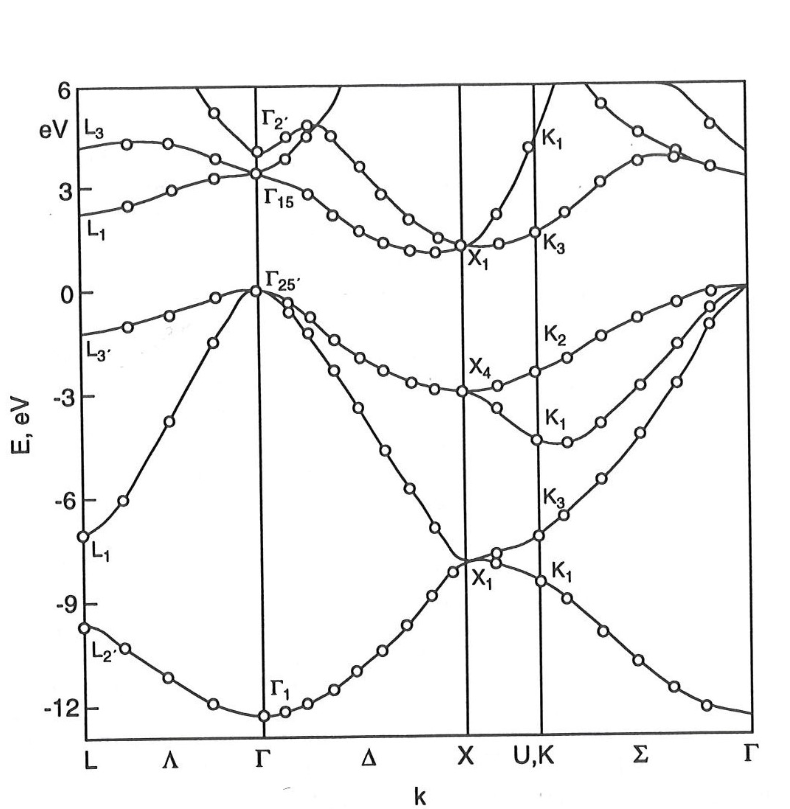
\includegraphics[width=0.5\textwidth]{sil_dispersion1.png}
    \caption{Dispersionsrelation von Silizium aus~\cite{silicon}.}
    \label{fig:sildisp}
\end{figure}

Siliziumdioxid $\mathrm{SiO}_2$ ist eines der am häufigsten vorkommenden Materialien auf der Erde, so besteht zum Beispiel Sand aus Siliziumdioxid, und ist auch als Quarz bekannt. Die wohl größte Bedeutung kommt Siliziumdioxid wohl als Glas zu, welches daraus hergestellt wird. Nicht wegzudenken ist es ebenso aus der Elektronikindustrie, da aus Siliziumdioxid unter Hitze und Zugabe eines Katalysators reines Silizium gewonnnen werden kann.